% Document Type Management
\documentclass{book}
\usepackage[utf8]{inputenc}
\usepackage[english]{babel}
 
 
 % Packages for Bibiography Management
\usepackage{biblatex}
\usepackage{csquotes}
\addbibresource{references.bib}

% AMS Packages
\usepackage{amsfonts}
\usepackage{amssymb}
\usepackage{amsmath}
\usepackage{amsthm}
\usepackage{esvect}

% Images Management Packages
\usepackage{tcolorbox}
\usepackage{graphicx}
\graphicspath{ {images/} }


% Packages to Draw Images
\usepackage{tikz}
\usetikzlibrary{shapes,backgrounds}
\usetikzlibrary{positioning}


% Custom Section Labels
\theoremstyle{definition}
\newtheorem{theorem}{Theorem}[section]
\newtheorem{corollary}{corollary}[theorem]
\newtheorem{lemma}[theorem]{Lemma}
\newtheorem{definition}[theorem]{Definition}
\newtheorem{example}[theorem]{Example}
\newtheorem{conjecture}[theorem]{Conjecture}

% Book Cover Page
\title{\textsc{MATHEMATICAL PROOF STRUCTURES}\\ {\bf Logic - Set Theory - Number Theory - Linear Algebra}\\ Scrap Work}
\author{Vernon V. Lallman}
\date{\today}

\begin{document}
 \maketitle

\tableofcontents

\newpage
\begin{definition}
Propositional Function \\
    
    A {\bf Propositional Function} (open sentence) is a sentence $P(x_1, x_2, \cdots, x_n)$ involving variables $x_1, x_2, \cdots, x_n$, then the resulting sentence is either true or false. That is, the resulting sentence is a statement. \\
    {\bf Notation:} One reason an open sentence is called a propositional function is the fact that we use function notation $P(x_1, x_2, \cdots, x_n)$ for an open sentence in $n$ variables. When there is only one variable, such as $x$, we write $P(x)$. In this notation $x$ represents an arbitrary element of the unviersal set, and $P(x)$ represents the sentence. When we substitute a specific element of the universal set $x$, the resulting sentence becomes a statement. \\
\end{definition}



\newpage
\section{TOPICS IN LOGIC}
\subsection{Statements and Conditional Statements}

\begin{definition}
Images Test \\

\begin{center}
    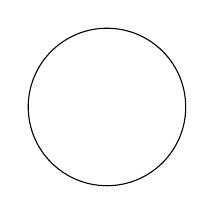
\begin{tikzpicture}
        \draw (0,0) circle (1cm);
    \end{tikzpicture}
\end{center}


%------------------------------------------------------------------------------
%Introductory example
\begin{figure}[p]
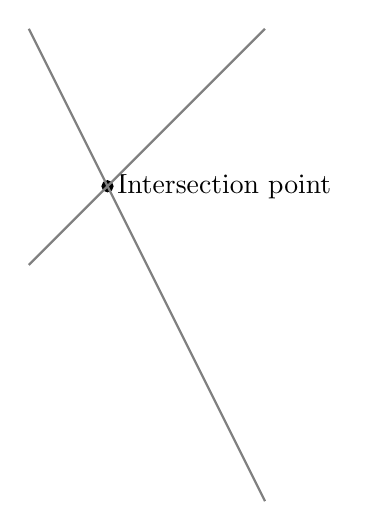
\begin{tikzpicture}
\filldraw[black] (0,0) circle (2pt) node[anchor=west] {Intersection point};
\draw[gray, thick] (-1,2) -- (2,-4);
\draw[gray, thick] (-1,-1) -- (2,2);
\end{tikzpicture}
\end{figure}
%------------------------------------------------------------------------------


%------------------------------------------------------------------------------
%Points, lineas and curves
\begin{figure}[p]
\begin{tikzpicture}
\draw (-2,0) -- (2,0);
\filldraw [gray] (0,0) circle (2pt);
\draw (-2,-2) .. controls (0,0) .. (2,-2);
\draw (-2,2) .. controls (-1,0) and (1,0) .. (2,2);

\end{tikzpicture}
\end{figure}
%------------------------------------------------------------------------------


%------------------------------------------------------------------------------
%Circles and arcs
\begin{figure}[p]
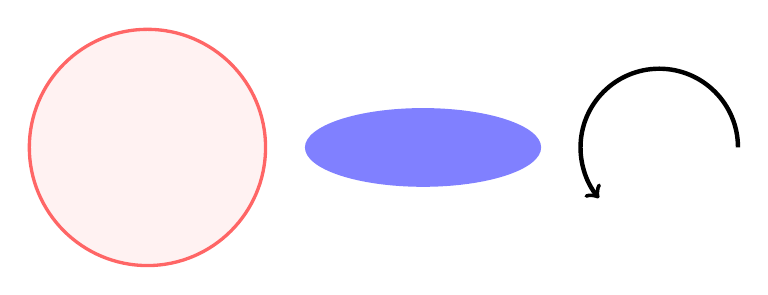
\begin{tikzpicture}
\filldraw[color=red!60, fill=red!5, very thick](-1,0) circle (1.5);
\fill[blue!50] (2.5,0) ellipse (1.5 and 0.5);
\draw[ultra thick, ->] (6.5,0) arc (0:220:1);
\end{tikzpicture}
\end{figure}
%------------------------------------------------------------------------------



%------------------------------------------------------------------------------
%Polygons
\begin{figure}[p]
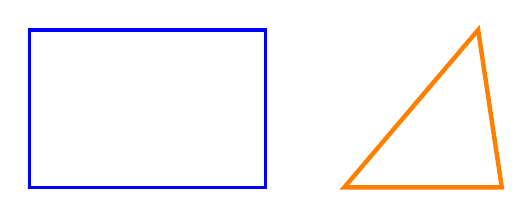
\begin{tikzpicture}
\draw[blue, very thick] (0,0)rectangle (3,2);
\draw[orange, ultra thick] (4,0) -- (6,0) -- (5.7,2) -- cycle;
\end{tikzpicture}
\end{figure}
%------------------------------------------------------------------------------


%------------------------------------------------------------------------------
%Diagram
\begin{figure}
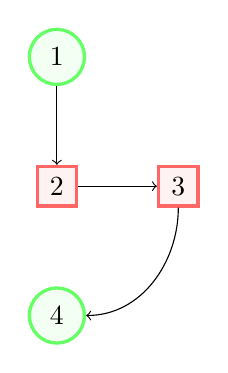
\begin{tikzpicture}[
roundnode/.style={circle, draw=green!60, fill=green!5, very thick, minimum size=7mm},
squarednode/.style={rectangle, draw=red!60, fill=red!5, very thick, minimum size=5mm},
]
%Nodes
\node[squarednode]      (maintopic)                              {2};
\node[roundnode]        (uppercircle)       [above=of maintopic] {1};
\node[squarednode]      (rightsquare)       [right=of maintopic] {3};
\node[roundnode]        (lowercircle)       [below=of maintopic] {4};

%Lines
\draw[->] (uppercircle.south) -- (maintopic.north);
\draw[->] (maintopic.east) -- (rightsquare.west);
\draw[->] (rightsquare.south) .. controls +(down:7mm) and +(right:7mm) .. (lowercircle.east);

\end{tikzpicture}
\end{figure}

%------------------------------------------------------------------------------


%------------------------------------------------------------------------------
%List of available colors 

\begin{figure}[p]

\begin{tikzpicture}
\filldraw[black] (0,0) rectangle (2,2);
\filldraw[red] (3,0) rectangle (5,2);
\filldraw[green] (6,0) rectangle (8,2);
\filldraw[blue] (9,0) rectangle (11,2);
\filldraw[cyan] (1,-1) rectangle (3,-3);
\filldraw[magenta] (4,-1) rectangle (6,-3);
\filldraw[yellow] (7,-1) rectangle (9,-3);
\end{tikzpicture}
\end{figure}
%------------------------------------------------------------------------------


%------------------------------------------------------------------------------
%Different levels of thickness
\begin{figure}[p]
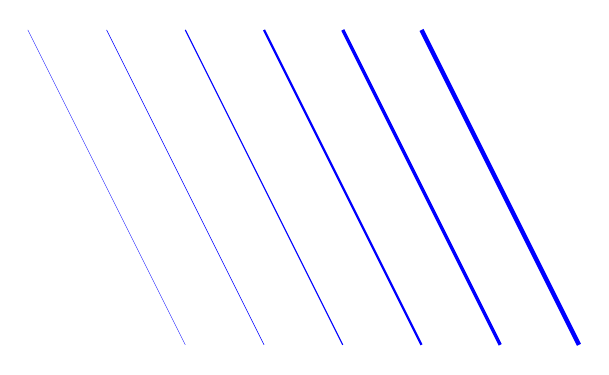
\begin{tikzpicture}
\draw[blue, ultra thin] (-1,2) -- (1,-2);
\draw[blue, very thin] (0,2) -- (2,-2);
\draw[blue, thin] (1,2) -- (3,-2);
\draw[blue, thick] (2,2) -- (4,-2);
\draw[blue, very thick] (3,2) -- (5,-2);
\draw[blue, ultra thick] (4,2) -- (6,-2);
\end{tikzpicture}
\end{figure}
%------------------------------------------------------------------------------




\end{definition}


\newpage
\begin{example}
Sequence Conjecture and Proof

To illustrate a proof which requires the extended first principle, Consider the \textbf{Lucas Sequence}:
    \begin{equation*}
        1, 3, 4, 7, 11, 18, 29, 47, 76, \cdots
    \end{equation*}
Except for the first two terms, each term of the sequence is the sum of the preceding two, so that the sequence may be defined inductively by:
    \begin{align*}
        a_1 & = 1 \\
        a_2 & = 3 \\
        a_3 & = 4 = 3 + 1 = a_2 + a_1 \\
        a_n & = a_{n-1} + a_{n-2} \text{, }\forall n \geqq 3 \\
    \end{align*}
We contend that the inequality $a_n < (\frac{7}{4})^n$ holds for every postive integer $n$. Now, let's formally prove this proposition: \\ 

Prove that every element $n$ of the lucas sequence is always less than ${\frac{7}{4}}^n$. 
\begin{tcolorbox}
    \begin{theorem}
        The following inequality holds for the \textbf{Lucas Sequence}, $1, 3, 4, 7, 11, 18, \cdots$
            \begin{equation*}
                1,3,4,7,11, \cdots \sum_{i \geqq 3}^{n}{ \left  \{ a_{i-1} + a_{i-2} \right \}}  < \left \{ \frac{7}{4}^{n} \middle |\ \forall n \in \mathbb{N} \right \}
            \end{equation*} 
    \end{theorem}
\end{tcolorbox}

\begin{proof}
        We will use a proof by the Extended First Principle of Mathematical Induction. For each natural number $n$, we let $P(n)$ be
            \begin{equation*}
                 1,3,4,7,11, \cdots \sum_{i \geqq 3}^{n}{ \left  \{ a_{i-1} + a_{i-2} \right \}}  < \left \{ \frac{7}{4}^{n} \middle |\ \forall n \in \mathbb{N} \right \}
            \end{equation*}
        We first prove that $P(1)$ and $P(2)$ is true. For the case, $P(1)$, notice that $a_1 < {\frac{7}{4}}^1$. This shows that   
            \begin{equation*}
                 1 < \frac{7}{4}
            \end{equation*}
        which proves that $P(1)$ is true. Similarly, we can see that $a_2 < {\frac{7}{4}}^2$. This shows that   
            \begin{equation*}
                 3 < \frac{49}{16}
            \end{equation*}
        Whence, the the inequality holds for both $P(1)$ and $P(2)$. This provides us the basis step for induction. \\ 
        
        For the inductive step, we prove that for all $k \in \mathbb{Z}$ with $k \geqq 3$, if $P(k)$, then $P(k+1)$. So let $k$ be a integer and assume that $P(k)$ is true. That is, we assume that 
            \begin{equation*}
               \sum_{i \geqq 3}^{k}{ \left  \{ a_{i-1} + a_{i-2} \right \}}  < \left \{ \frac{7}{4}^{k} \middle |\ \forall k \in \mathbb{N} \right \}
            \end{equation*}
        
        The goal is to prove that $P(k+1)$ is true. That is, it must be proved that  
            \begin{equation}
            \label{dneg}
                \sum_{i \geqq 3}^{k}{ \left  \{ a_{i-1} + a_{i-2} \right \}}  < \left \{ \frac{7}{4}^{k} \middle |\ \forall k \in \mathbb{N} \right \}
            \end{equation}
        
        To do this, will add the $k-1$ and $k-2$ elements on both sides of the equation (\ref{dneg}) and algebraically rewrite the right hand side of the resulting equation. This gives
            \begin{align*}
                \sum_{i \geqq 3}^{k}{ \left  \{ a_{i-1} + a_{i-2} \right \}} & < \frac{7}{4}^{k-1} + \frac{7}{4}^{k-2} \\
                    & < \frac{{\frac{7}{4}}^4}{\frac{7}{4}} + \frac{{\frac{7}{4}}^4}{{\frac{7}{4}}^2} \\
                    & < \frac{{\frac{7}{4}}^{2k} + {\frac{7}{4}}^k}{{\frac{7}{4}}^2} \\
                    & < \frac{{\frac{7}{4}}^{3k}}{{\frac{7}{4}}^k} \\
                    & < {\frac{7}{4}}^k \\
            \end{align*}
        
        Hence, the inductive step has been established, and by the Extended First Principle of Mathematical Induction, we have proven that the inequality holds true for $n=k$ whenever it is true for then natural numbers, we conclude by the extended first principle that
            \begin{equation*}
                1,3,4,7,11, \cdots \sum_{i \geqq 3}^{n}{ \left  \{ a_{i-1} + a_{i-2} \right \}}  < \left \{ \frac{7}{4}^{n} \middle |\ \forall n \in \mathbb{N} \right \}
            \end{equation*}
\end{proof}
\end{example}



\newpage
\begin{example}
Suppose $n$ is an natural number and $x_1, x_2, \cdots x_n, y_1, y_2, \cdots y_n$ are $(2n)$ real numbers then prove the following theorem:
    
    \begin{tcolorbox}
        \begin{theorem}
            For each natural number $x$ and $y$,
                \begin{equation*}
                    \sum_{k=1}^{n}{x_k + y_k} = \sum_{k=1}^{n}{x_k} + \sum_{k=1}^{n}{y_k}                
                \end{equation*}
        \end{theorem}
    \end{tcolorbox}

    \begin{proof}
        We will use the first principle of finite induction. For this proof, we let
            \begin{equation*}
                P(n) \text{ be } {k=1}^{n}{x_k + y_k} = \sum_{k=1}^{n}{x_k} + \sum_{k=1}^{n}{y_k} 
            \end{equation*}
        We first prove that $P(1)$ is true. Using $n=1$, we see that
            \begin{equation*}
                x_1 + y_1 = \sum_{k=1}^{n}{x_k} + \sum_{k=1}^{n}{y_k}  = \sum_{k=1}^{1}{x_1} + \sum_{k=1}^{1}{y_1}  = x_1 + y_1
            \end{equation*}
        This means that $\sum_{k=1}^{1}{y_1}  = x_1 + y_1$, and hence $P(1)$ is true. \\
        For the inductive step, we prove that for all $q \in \mathbb{N}$ with $q \geqq 1$, 
            \begin{center}
                If $P(q)$, then $P(q+1)$
            \end{center}
        So let $q$ be a natural number greater than or equal to unity, and assume that $P(q)$ is true. That is, assume that 
            \begin{equation*}
               \sum_{k=1}^{q}{x_k + y_k} = \sum_{k=1}^{q}{x_k} + \sum_{k=1}^{q}{y_k}
            \end{equation*}
        The goal is to prove that $P(q+1)$ is true. To obtain the sum to $q+1$ element, we merely add the next one, $x_q+1 + y_q+1$, to both sides of the equation. This gives: 
            \begin{align*}
                \sum_{k=1}^{q+1}{x_k + y_k} & = \sum_{k=1}^{q}{x_k} + \sum_{k=1}^{q}{y_k} + x_q+1 + y_q+1 \\
                    & =  \left [ \sum_{k=1}^{q}{x_k} + x_q+1 \right ]  + \left [ \sum_{k=1}^{q}{y_k} + y_q+1 \right ] \\
                    & =  \left [ \sum_{k=1}^{q+1}{x_k} \right ]  + \left [ \sum_{k=1}^{q+1}{y_k} \right ] \\
            \end{align*}
        and this proves that if $P(k)$ is true then $P(k+1)$ is true. Thus, the inductive step has been established, and so by the first principle of finite induction,
            \begin{equation*}
                 \sum_{k=1}^{n}{x_k + y_k} = \sum_{k=1}^{n}{x_k} + \sum_{k=1}^{n}{y_k} 
            \end{equation*}
    \end{proof}
\end{example}








\end{document}